\begin{savequote}
Gesture is a critical link running through the evolution of perception,
conceptualization, and language.
\qauthor{David Armstrong, William Stokoe, and Sherman Wilcox, \textit{Gesture
and the nature of language}}
\end{savequote}
\chapter{Introduction}
% (Start with a motivating scenario: either Powerpoint presentation or USAR
% application.)
% \begin{quotation}
% \textit{Imagine an earthquake has hit a populous area and many major roads are
% impassable. Buildings are severely damaged or collapsed, and fire has broken out
% in many places. At the crisis management center, response professionals are
% working together to coordinate the earthquake relief effort. You are the
% incident commander charged with coordinating the search
% and rescue teams working in the field. There is a large tabletop display in
% front of you, showing the map of the site. Information coming from the field is
% updated on the display in real-time.}
% 
% \textit{A report about a big explosion at a chemical plant comes in and you move
% the map around, zoom in and rotate it to get a good view of the plant. On the
% map, you see there is a group of unmanned vehicles nearby. After selecting them
% on the map with your hand, you speak to the interface ``Go nearer to the
% explosion site to gather more information,'' while tracing the route the
% vehicles should take to avoid obstacles. Then you instruct rescue team No. 3 to evacuate the residents
% in the surrounding buildings by going under a bridge because the surface of the
% bridge is blocked. You gesture with one hand as the bridge and the other
% hand moving under it to emphasize this.}
% \end{quotation}
% 
% The scenario above is an example in the Urban Search and Rescue (USAR) domain.
% It shows an application of a multi-modal interface to a real-world problem. Gestures play an important part in this scenario,
% providing key information about location, method and timing of movements,
% and about spatial relationship among the objects being described.
\begin{quotation}
Imagine how nice it would be, the next time you make a presentation, if you did not need to stand close to your laptop or use a remote control with its limited functionality. What if you could present your work as naturally as having a conversation with your audience. You swipe your hand left and right to change slides. When you point to the slide with your hand, the display shows a pointer cursor following wherever you point. When you are showing a video, you use a palm forward hand pose (�stop� gesture) to pause the movie, then move left and right to fast forward or rewind the video. You can also say �faster� or �slower� to change the video speed. When you need to jump to a particular slide, you make a circle gesture to show all the slides, and say "show this slide'' while pointing at that slide. You can also make a dismiss gesture to pause the slide show (making the screen black) to take the distracting slides off the screen and get full attention from the audience during presentation.

\end{quotation}

The above scenario shows an application of a multimodal interface to a
real-world problem, with different types of gestures playing an important part
in the scenario. The system I developed makes the scenario real. It provides real-time continuous gesture recognition and interaction, addressing problems that have previously been neglected, such as handling different types of gestures, and determining how and when the system should respond. 

 
Recent trends in user interfaces have brought on a new wave of interaction
techniques that depart from the traditional mouse and keyboard that have been 
used for decades. These include multi-touch interfaces such as the 
iPhone, the iPad and the Microsoft 
Surface\textsuperscript{\textregistered} as well as camera-based systems such as
the Microsoft Kinect and the Leap Motion sensor. Most
of these devices gained instant popularity among consumers, and the common trait
among them is that they make interacting with computation more natural and 
effortless. All these devices allow users to use their hands and/or body 
gestures to directly manipulate virtual objects. It feels more natural this 
way because this is how we interact with our environment in everyday life.
 
There is also a trend in wearable human-computer interfaces recently pioneered
by products such as Google Glass, Samsung's Galaxy Gear smartwatches and Pebble
smartwatches. These products have potential for gesture input as well. Google
Glass has a camera which can be used to recognize hand motion and hand shapes.
The accelerometers in the smartwatches can also be used to measure hand motion,
just like the Nintendo Wii controller.

There are big potential and demand for natural interaction, and gesture is
an important part of it. We start to see more and more gestural interfaces,
however, many of them still mainly make the hands function as a mouse with a
limited number of other gestures. Our goal is to break out from the old
paradigm of ``point, click, drag'' interaction we used to have with mice. 
Our hands are much more versatile, and hence, I believe that to design a gesture
recognition system for natural human computer interaction (HCI), we need to
start from the user interaction perspective: what are the different types of
gestures people use; when should the system respond; how should the model be
defined and trained; and how to combine gesture and speech for natural
interaction. These are the questions I addressed in this thesis. Based on my
findings, I developed a real-time continuous gesture recognition and
interaction system that handles different types of gestures seamlessly, and
responds to gestures appropriately.

\section{Background}
To design a natural gestural interface, it is important to understand the
nature of human gestures. This section gives some background information in
gesture production and taxonomy, and introduces several important concepts and
terms that are central to the final system design.
 
\subsection{Definition of Gestures}
Webster's Dictionary defines gestures as ``\ldots a movement usually of the body or limbs
that expresses or emphasizes an idea, sentiment, or attitude.'' This definition
is particularly related to the communicative aspect of the human hand and body
movements. However, in HCI, the notion
of gestures is somewhat different. In their review of the visual interpretation
of hand gestures for HCI, Pavlovic et al. \cite{Pavlovic97} state that in a computer
controlled environment one wants to use the human hand to perform tasks that
mimic both the natural use of the hand as a manipulator, and its use in
human-machine communication. They include both \textit{manipulative} and
\textit{communicative} gestures in their gesture taxonomy. This is also the
definition I use in the thesis.

\begin{figure}[tbh]
  \centering
  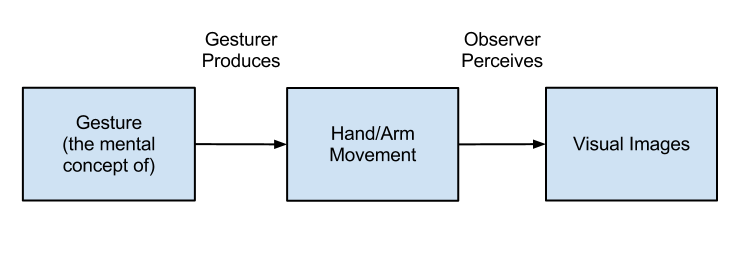
\includegraphics[width=0.7\textwidth]{figures/gesture_production.png} 
  \caption{Production and perception of gestures. Hand gestures originate as a
  mental concept, are expressed through arm and hand motion, and are perceived
  as visual images \cite{Pavlovic97}.}
  \label{fig:gesture_production}
\end{figure}

Pavlovic et al. \cite{Pavlovic97} also gives a model (Figure. 
\ref{fig:gesture_production}) for the production and perception of gestures 
based on the model used in the field of spoken language recognition. According 
to their model, gestures originate as a gesturer's mental concept, possibly in 
conjunction with speech. They are expressed through the motion of arms and 
hands. Also, observers perceive gestures as streams of visual images which they
interpret using their knowledge about those gestures. In HCI, the 
observer is the computer and the knowledge it possesses is the training data.

\subsection{Gesture Taxonomy for Natural Interaction}\label{sec:taxonomy}
Several gesture taxonomies have been suggested in the literature. Some of them
deal with psychological aspects of gestures \cite{kendon86, mcneill82}, while
others are inspired by an HCI perspective \cite{Pavlovic97, quek95, wobbrock09}. 
The taxonomy that seems most appropriate for natural HCI and human-centric
design is developed by Wobbrock et al.~\cite{wobbrock09}. Their study is based on
eliciting natural behavior from non-technical users when interacting with a computing system.
As their user study focuses on tabletop gestures, I further generalize the
taxonomy to encompass interaction for both vertical and horizontal interfaces.

Wobbrock et al. \cite{wobbrock09} classified gestures into four
orthogonal dimensions: \textit{nature}, \textit{form},
\textit{flow}, and \textit{binding}. Among the four dimensions, the nature
dimension is the mostly widely used in other related work, and hence, it is
worth further explanation.
The form dimension is particularly relevant for building the gesture recognition model because
different forms constitute different features we need to consider. The binding and the flow
dimensions are relevant for the application layer because they are related to
how the user interface should respond to gesture events.

\subsubsection{Nature of Gestures}
\begin{figure}[tbh]
  \centering
  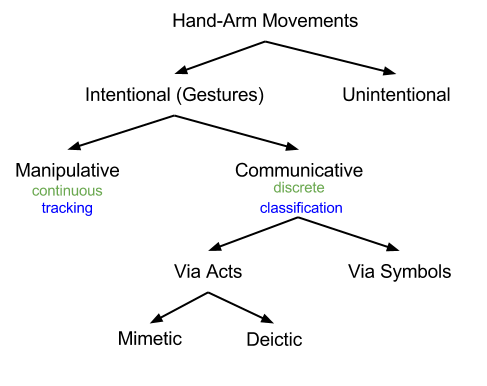
\includegraphics[width=0.5\textwidth]{figures/taxonomy.png} 
  \caption{Hierarchical classification of gestures in the nature dimension.}
  \label{fig:taxonomy}
\end{figure}

The hierarchical taxonomy by Pavlovic et al.~\cite{Pavlovic97} gives
a comprehensive categorization of gestures in the nature dimension (Figure
\ref{fig:taxonomy}).
First, gestures, as \textit{intentional} movements, should be distinguished from \textit{unintentional} hand movements, i.e., \textit{non-gestures}.
Unintentional movements are movements that are not intended to convey
information. In contrast, gestures are meaningful hand movements that people make to convey some
information. The distinction is important for a natural interface because there
should not be any restriction on how people should place or move their hands
when they are not doing any meaningful gestures.  


Gestures are then further divided into manipulative and communicative
categories. Manipulative gestures are used to act on objects (e.g.
moving an virtual object around, click a button, the property of the virtual
object change directly according to certain parameters of the hand(s)), while
communicative gestures have an inherent purpose for communication \cite{Pavlovic97}. 

People perform communicative gestures via acts or symbols. Gesture via acts are
those directly related to the interpretation of the movement itself. Such
movements are classified as either mimetic (which imitate some actions) or
deictic (pointing acts that convey spatial information). Gestures via symbols
are those that have a linguistic role, and are often represented by different static hand postures. An example is forming the
O.K. pose for ``accept''. 

\subsubsection{Gesture Forms and Flows}
The forms and the flows dimensions (see Table~\ref{tab:taxonomy}) are the focus of this
thesis.

\begin{table}[tbh]
\centering
\begin{tabular}{|c|l|l|}
\hline
\multirow{2}{*}{\textbf{\textit{Form}}} & \textit{distinct path} & with any hand
pose
\\
\cline{2-3} 
                               & \textit{distinct hand pose} & with any path \\
\hline
\multirow{2}{*}{\textbf{\textit{Flow}}} & \textit{discrete} & response occurs
\textit{after} the user acts \\
\cline{2-3}
              & \textit{continuous} & response occurs \textit{while} the user
              acts \\
\hline
\end{tabular}
\caption{Gesture forms and flows.}
\label{tab:taxonomy}
\end{table}

I distinguish two
categories in the form dimension: \textit{path} and \textit{pose}. The path
category contains gestures characterized by distinct paths without any distinct
hand poses. For example, a ``swipe left'' gesture is characterized by a
right to left motion, while a ``circle'' gesture is characterized by a
circular motion of the hand. In doing these, users typically hold their
hands in some natural, relaxed, but unpredictable pose. Pose
gestures are characterized by distinct hand poses without any distinct paths.
This category of gestures is usually associated with direct manipulation of some virtual
objects on the interface.
For example, a user may use a ``point'' hand pose and move around to
point at different things on a display.

In the flow dimension, a gesture's flow is
\textit{discrete} if the gesture is performed, delimited, recognized, and
responded to as an atomic event~\cite{wobbrock09}. For example, if the ``wave'' gesture is
regarded as a discrete flow gesture, the system should respond once at the last
repetition of the left-right motion. Flow is \textit{continuous} if ongoing
recognition is required and the system should respond frame by frame, as for example during a ``point'' gesture, where we want to show the cursor on the screen
continuously moving according to the hand position. 

\subsection{Temporal Modeling of Gestures}
Making gesture interaction feel natural requires a system to respond at the
correct moment. As a result, it is important to consider the temporal
characteristics of gestures. We set a foundation for doing this by taking
account of the three phases that make of a gesture:
\begin{itemize}
  \item pre-stroke,
  \item nucleus (peak \cite{mcneill82}), and
  \item post-stroke \cite{Pavlovic97}.
\end{itemize}
``Pre-strokes'' and ``post-strokes'' are movement from and to the
rest position. The ``nucleus'' of a gesture,
as Kendon \cite{kendon86} observes, has some ``definite form and enhanced dynamic
qualities''. Every gesture must have a nucleus, which is the content-carrying
part of the gesture. Based on this theory, the lack of the nucleus phase can
be used to filter out unintentional movements from gestures .

Even though the end of the
post-stroke phase can be more easily detected by finding the start of the
rest position, we want to do more than this. Since the nucleus phase is the
meaningful part of the gesture, for a discrete flow gesture, we want the system to respond immediately at the end of the nucleus
 instead of at the end of the post-stroke. To make the system more responsive,
I address the more challenging problem of detecting the start and end of the
 nucleus phase from the pre-stroke and post-stroke phases. This also allows the system to respond to continuous
flow gesture immediately at the start of the nucleus phase.

\section{System Overview and Thesis Outline}
The gesture interaction system consists of four modules: hand tracking, 
feature extraction, gesture recognition, and application user interface
(Figure~\ref{fig:overview}). At each time frame, the
hand tracking module takes raw data from the sensor and estimates the location
of the gesturing hand. The feature extraction module computes feature
descriptors from the localized hand and sends the encoded features to the
gesture recognition module.
The gesture recognition model estimates the current most likely gesture label and gesture phase information based on the input stream of
feature vectors. The gesture information, 
together with smoothed hand position information are sent to the application
level. 

\begin{figure}[tbh]
\centering
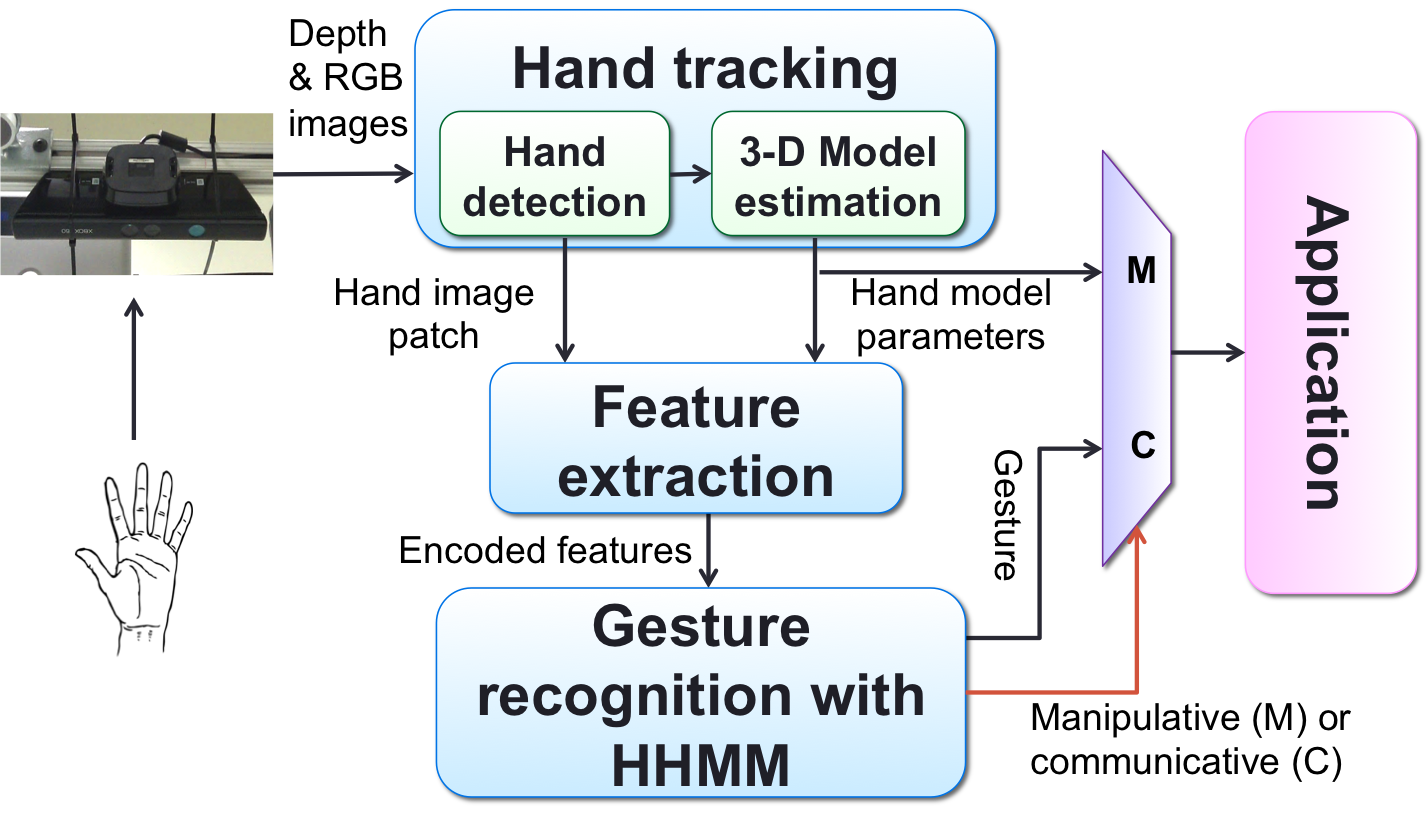
\includegraphics[width=0.7\linewidth]{figures/system_overview.png}
\caption{System overview.}
\label{fig:overview}
\end{figure}

In each module, I have improved upon existing methods, and developed new
techniques to improve the gesture recognition accuracy and user experience. The main focus and contributions are in the gesture
recognition part. The thesis describes the methods used in each module in
detail. Please refer to Appendix~\ref{app:notation} for an explanation of
notation and a list of abbreviations.

\section{Contributions}
The main contributions of this work include:
\begin{itemize}
 \item Hand tracking
  \begin{itemize}
  \item Improved hand tracking methods based on gesture salience: I define
  gesture salience to be proportional to the amount of motion and the closeness
  of the motion to the observer. Based on this, I compute a probability map for the gesturing hand locations in a frame.  Compared with using the hand joint position from the Kinect SDK, using our hand tracking method gives a 3.7\% absolute increase in the recognition F1 score.
  \end{itemize}
 \item Feature extraction
  \begin{itemize}
  \item I use histogram of oriented gradients (HOGs) as a hand shape descriptor
  and apply principal component analysis (PCA) to reduce its dimensionality. I
  then use it as part of the feature vector input to the hidden Markov models (HMMs) based recognition module. This technique gives comparable recognition results to Support Vector Machine (SVM) which was commonly used before, and allows us to handle path and pose gestures in a unified way.
  \end{itemize}
  \item Gesture recognition
    \begin{itemize}
    \item Developed a probabilistic framework based on HMMs for real-time
    continuous (i.e., unsegmented) gesture recognition that unifies recognition
    of two forms of gestures (path and pose). I use different HMM topologies for
    different forms of gestures and combine them into one flattened HMM for
    simultaneous recognition and segmentation.
    \item Used embedded training and hidden state information to detect
    different gesture phases -- the pre-stroke, the nucleus, and the post-stroke
    phases -- allowing the system to respond more appropriately and promptly to
    gestures that require a discrete response and those needing a continuous response.
    \item Collected a new dataset (YANG dataset) that includes two forms of
    gestures (4 path and discrete flow gestures and 3 pose and continuous flow gestures from 10 users), a combination currently lacking in the community, to evaluate system performance.
    \item Developed a hybrid evaluation metric that is more relevant to
    real-time interaction with different gesture flows. With user dependent
    training and testing, we achieve an average F1 score of 0.805 (0.93 for discrete flow gestures and 0.68 for continuous flow gestures) on the YANG dataset.
    \item Used gesture phase information to do gesture spotting, filtering out
unintentional hand movement with no nucleus phases.
  \end{itemize}
  \item User interaction techniques
  \begin{itemize}
  \item Identified two main ways of  combining gesture and speech for natural
  interaction: using gestures to augment speech, and using speech to augment gestures. Demonstrated the combinations in an interactive system.
  \end{itemize}
\end{itemize}

% \subsection{Discriminative Training}
% HMMs as a generative model allows us to model the joint
% distribution of the observed sequence. Traditionally,
% maximum-likelihood (ML) estimation is used to learn the parameters of HMMs. However, our real task is to
% classify the sequence of the observed data. Discriminative classifiers model the
% posterior $p(y|x)$ directly, and hence are believed to give a lower error rate.
% In the speech recognition community, discriminative training methods have been
% proposed and have shown significant improvements over ML-trained models on many
% large vocabulary speech recognition tasks \cite {chang12}. To further improve
% the discriminative power of our model, we will use discriminative training
% methods for gestural analysis.
% 
% HMM provides a computationally efficient modeling framework. The HMM makes two
% main assumptions:
% 
% 1. There exists a hidden state sequence, $S$, that forms a Markov chain that
% generates the observation vectors.
% 
% 2. Given the state $s_t$ at any time point, the corresponding observation $x_t$
% is conditionally independent of other observations and states.
% 
% Instead of seeking model parameters that can maximize the likelihood of the
% data, discriminative training methods seek parameters that can minimize the
% confusions that occur in the training data. In general, discriminative training
% methods consist of two steps: First, construct a smooth and efficient computable
% objective function that reflects the degree of confusion; second, adjust the
% model parameters such that the objective function can be optimized. 
% 
% We will explore several commonly used discriminative training criteria such as
% minimum classification error training, maximum mutual
% information training, and margin-based training methods. For optimizing
% parameters, we can use either the extended Baum-Welch method or gradient-based
% methods. We will also compare the results to those without discriminative
% training and those with CRF-based models.

% \section{Appendix A - Review of Kalman Filter}
% Let $x_k$ be an $n$-dimensional vector of state components and $P_k$ be the
% $n$-by-$n$ error covariance. The measurement $z_k$ is an $m$-dimensional
% vector given by:
% \begin{align*}
% z_k = H_kx_k + v_k,
% \end{align*}
% where $H_k$ is an $m$-by-$n$ matrix and $v_k$ is the measurement error.
% 
% The \textit{Kalman gain}, $K_k$, is an $n$-by-$m$ matrix expressed as:
% \begin{align*}
% K_k = P_k^-H_k^T(H_kP_k^-H_k^T + R_k)^{-1}
% \end{align*}
% 
% Assuming no external control, the a priori estimate $x_k^-$ of the state is
% given by:
% \begin{align*}
% x_k^- = Fx_{k - 1} + w_k,
% \end{align*}
% where $F$ is the $n$-by-$n$ \textit{transfer matrix} characterizing the
% dynamics of the system, and $w_k$ is the \textit{process noise} associated with
% random events or forces that directly affect the actual state of the system. We assume that the components of $w_k$
% have Gaussian distribution $N(0, Q_k)$ for some $n$-by-$n$ covariance matrix
% $Q_k$.
% 
% Using $P_k^-$ to denote the error covariance, the a priori estimate for this
% covariance at time $k$ is obtained from the value at time $k - 1$ by:
% \begin{align*}
% P_k^- = FP_{k - 1}F^T + Q_{k - 1}
% \end{align*}
% 
% The updated value for $x_k$ when a new measurement is available is:
% \begin{align*}
% x_k = x_k^- + K_k(z_k^- - H_kx_k^-)
% \end{align*}
% The update value for $P_k$ is:
% \begin{align*}
% P_k = (I - K_kH_k)P_k^-
% \end{align*}
% 

